\section{The Existing System}
OpenSCAD in its present form applies the compile and render process sequentially in one thread of a process. The whole process begins when the user write (or completes) the textual description of their model and chooses to either just compile it or complie and render it one go (F6). The textual description of the language is taken through the following stages sequentially.
\begin{enumerate}
	\item The descriptional language is scanned, tokenized and converted into an Abstract Syntax Tree (AST). This is much like what any compiler does initially.
	\item The AST is converted into an Abstract Node Tree. This consists of the nodes that are to become the part of the final model.
	\item The node tree is fed to the CSGEvaluator which generates a preview of the model abstracting finer details.
	\item The final rendering of the model is done by the GeometryEvaluator.
\end{enumerate}

\begin{figure}
\centering
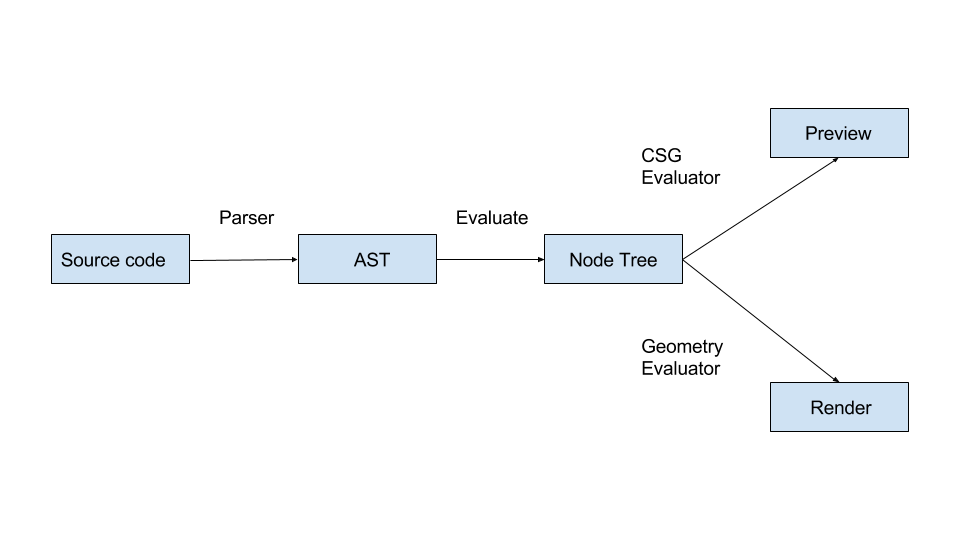
\includegraphics[width=0.7\linewidth]{images/flowchart}
\caption{}
\label{fig:flowchart}
\end{figure}

The present system is a bit slow in terms of its usage of the available CPU power. In being a single threaded process, everything has to happen in a sequence. This is not something which is required all the time. For example, during the evaluation of the node tree, various nodes can be evaluated in parallel in separate threads. Similarly at the time of rendering, this parallelism can be achieved.

{\bf {Limitations of previous system }}
\begin{itemize}
	\item Not utilizes the full potential of the CPU.
	\item The rendering process is very slow.
	\item When the user accidentely presses F6, there is no way to cancel that process and the user has to wait for the rendering to finish in order to continue their work.
	\item The system hangs frequently for more complex models on normal computers.
	\item It uses large amount of system resources. Their can be a significant improvement in this.
\end{itemize}
